\documentclass[tikz]{standalone}

\usepackage{kotex} 
\usepackage[english]{babel}
\usepackage{tikz}
\usepackage{textcomp}

\definecolor{sasaki}{HTML}{EF9AAF}
\definecolor{gibara}{HTML}{FFBE5C}
\definecolor{warabeda}{HTML}{E34E4F}
\definecolor{roa}{HTML}{D8368D}
\definecolor{toko}{HTML}{9D3757}
\definecolor{debiru}{HTML}{444C7D}

\begin{document}
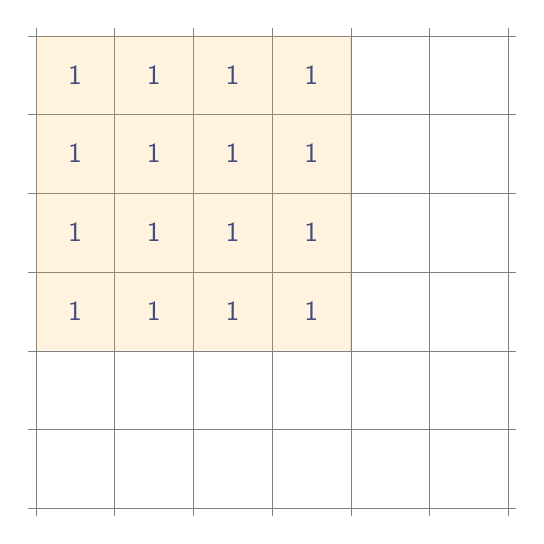
\begin{tikzpicture}
    \draw[step=1cm,gray,ultra thin] (-3.1, -3.1) grid (3.1, 3.1);
    
    \draw[step=1cm, draw=gray, ultra thin, fill=gibara, opacity=0.2] (-3, 3) grid (1, -1) rectangle (-3, 3);
    
    \foreach \x / \y in {-2.5/1, -1.5/1, -0.5/1, 0.5/1}
        \draw (\x, 2.5) node[debiru] {\textsf{\y}};
    \foreach \x / \y in {-2.5/1, -1.5/1, -0.5/1, 0.5/1}
        \draw (\x, 1.5) node[debiru] {\textsf{\y}};
    \foreach \x / \y in {-2.5/1, -1.5/1, -0.5/1, 0.5/1}
        \draw (\x, 0.5) node[debiru] {\textsf{\y}};
    \foreach \x / \y in {-2.5/1, -1.5/1, -0.5/1, 0.5/1}
        \draw (\x, -0.5) node[debiru] {\textsf{\y}};
    
\end{tikzpicture}
\end{document}
